\mychapter{5}{Задание №5}

Значение регистра \textbf{x31} на момент окончания выполнения программы равно 9, как предполагалось ранее.

\begin{center}
\centering 
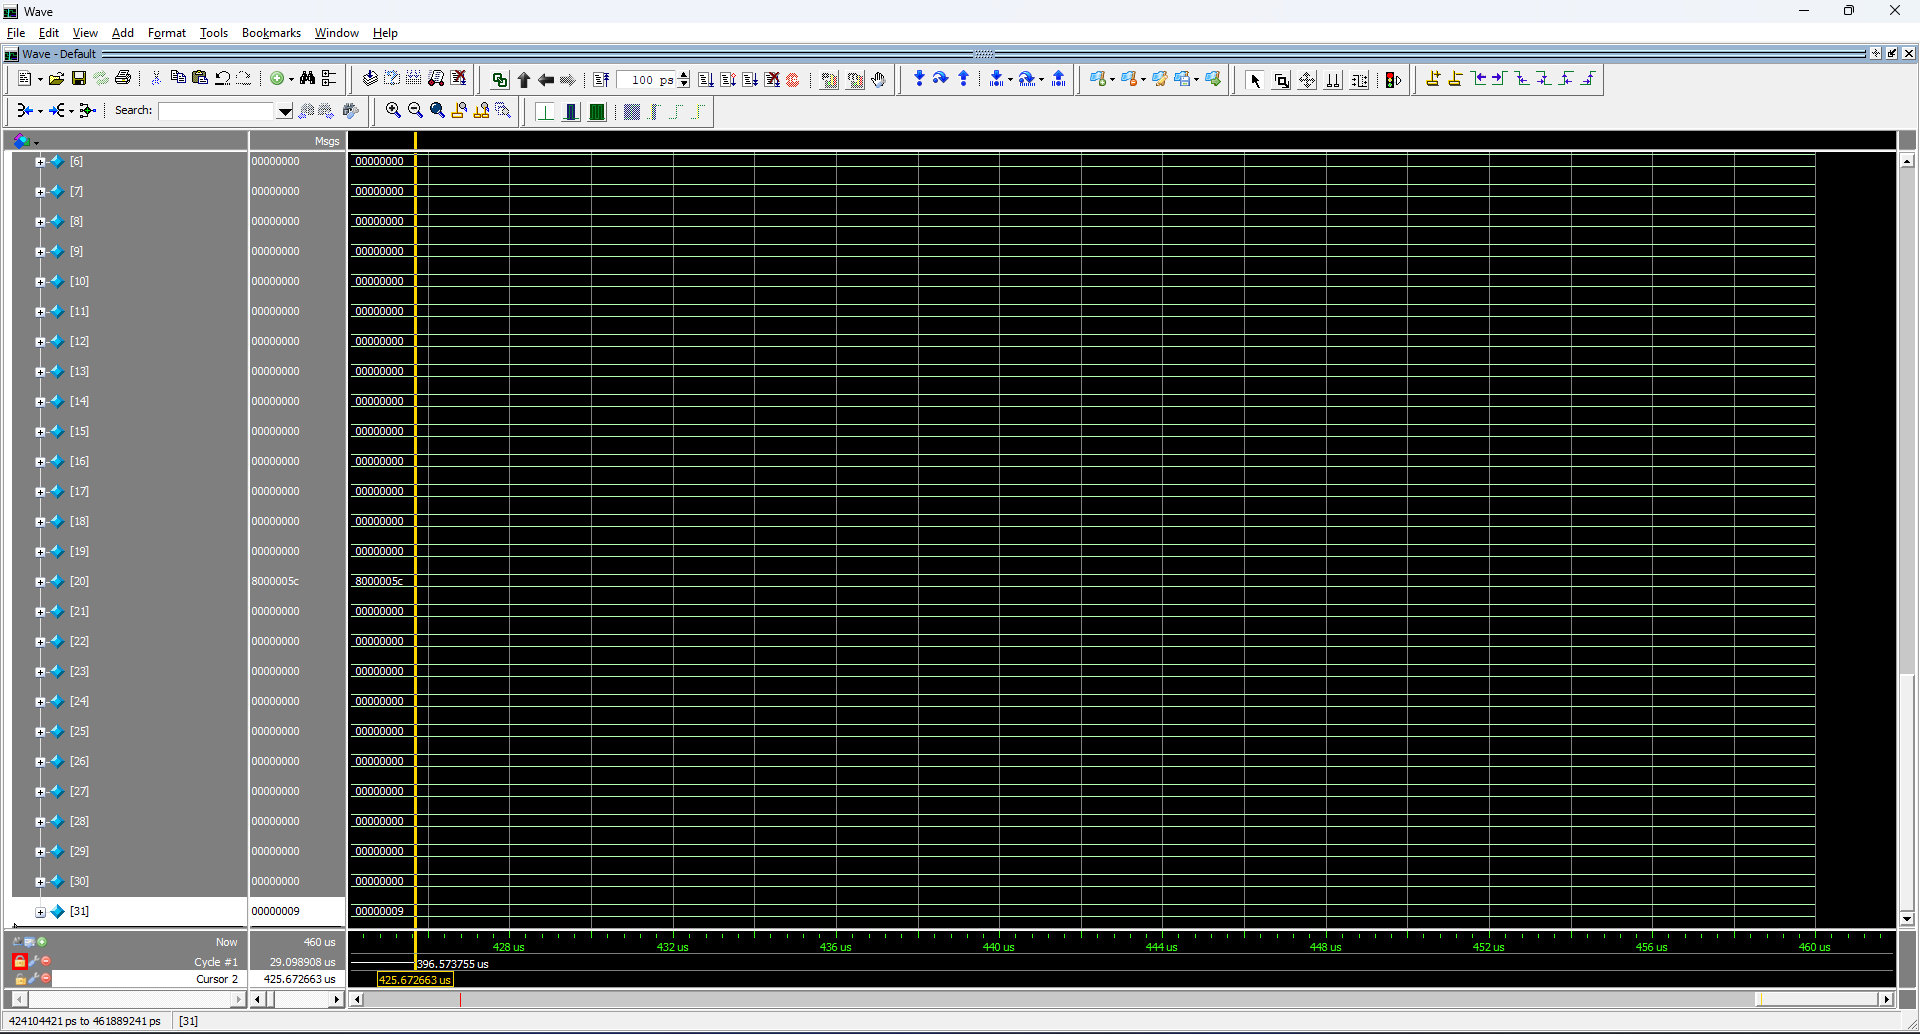
\includegraphics[scale=0.25]{images/05-x31_finally.png}
 \captionof{figure}{Значение регистра x31 на момент окончания выполнения программы}
\end{center}

\begin{center}
\centering 
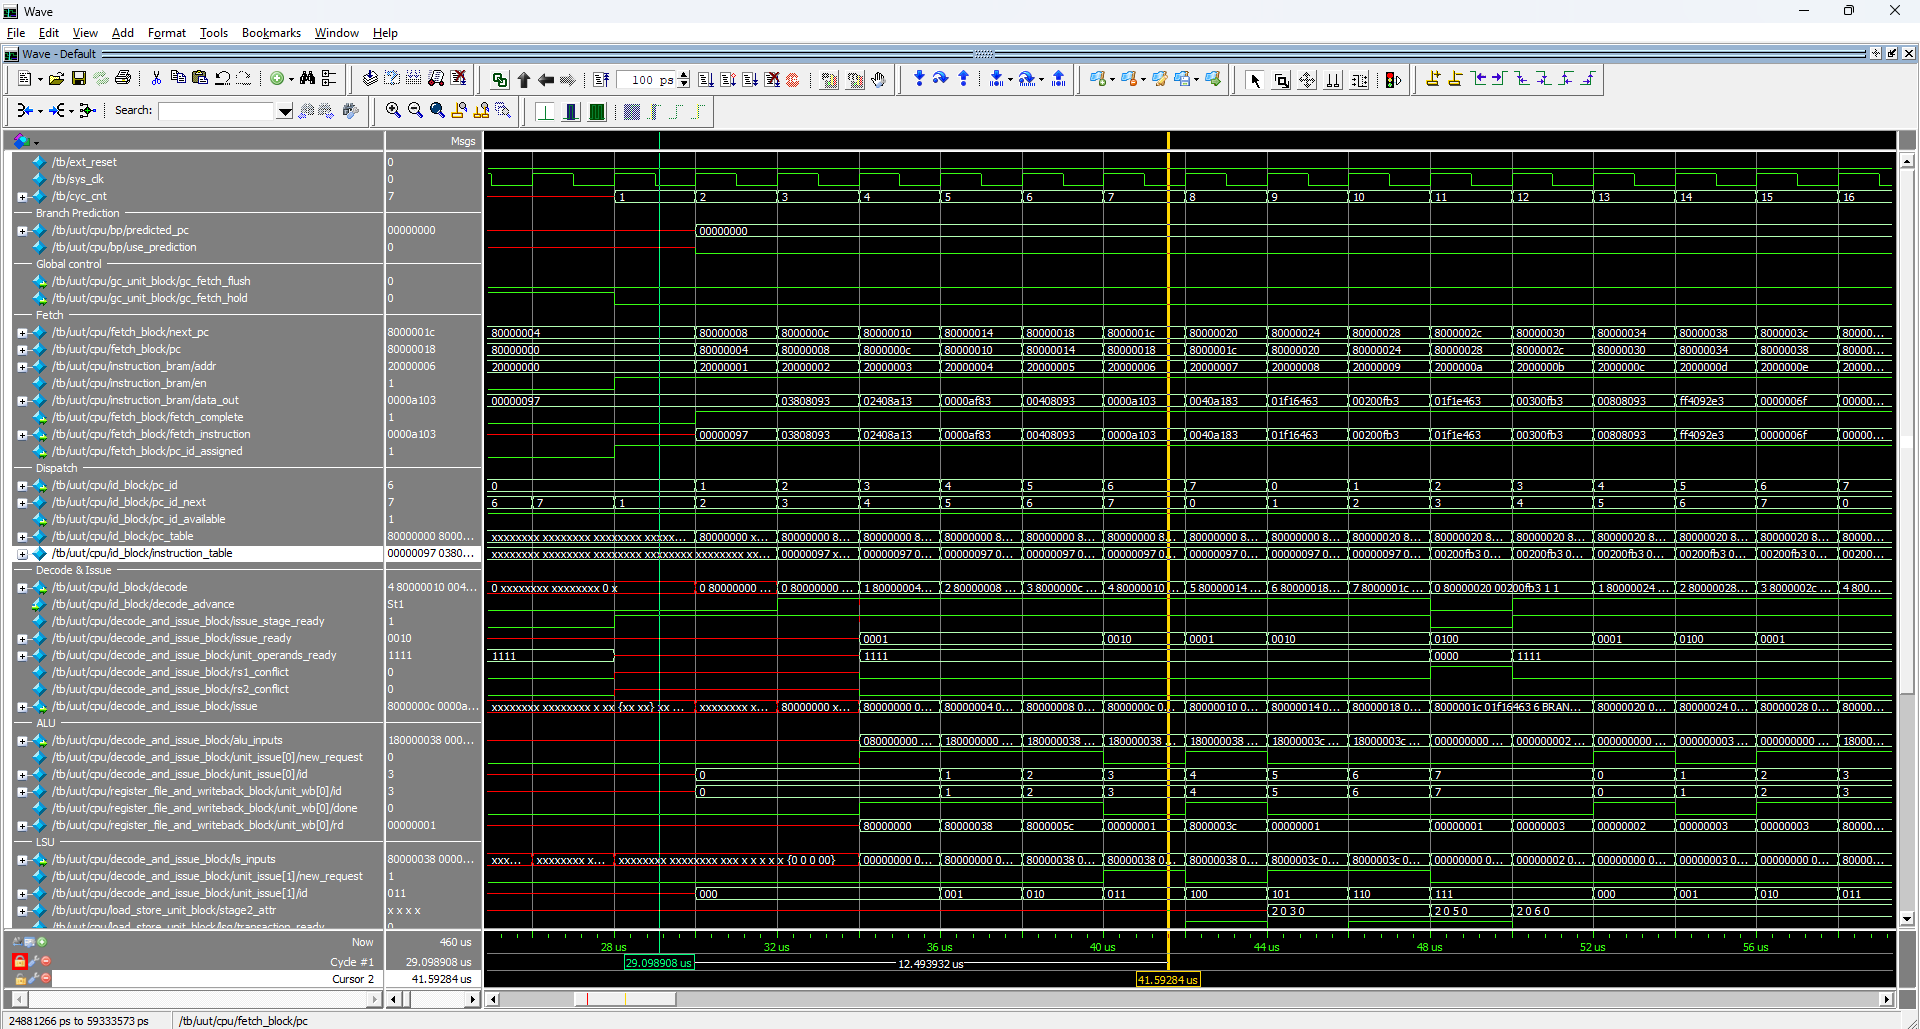
\includegraphics[scale=0.25]{images/05-fetch.png}
 \captionof{figure}{Временная диаграмма сигналов команды lw x3, 4(x1) на стадии выборки и диспетчеризации}
\end{center}

\begin{center}
\centering 
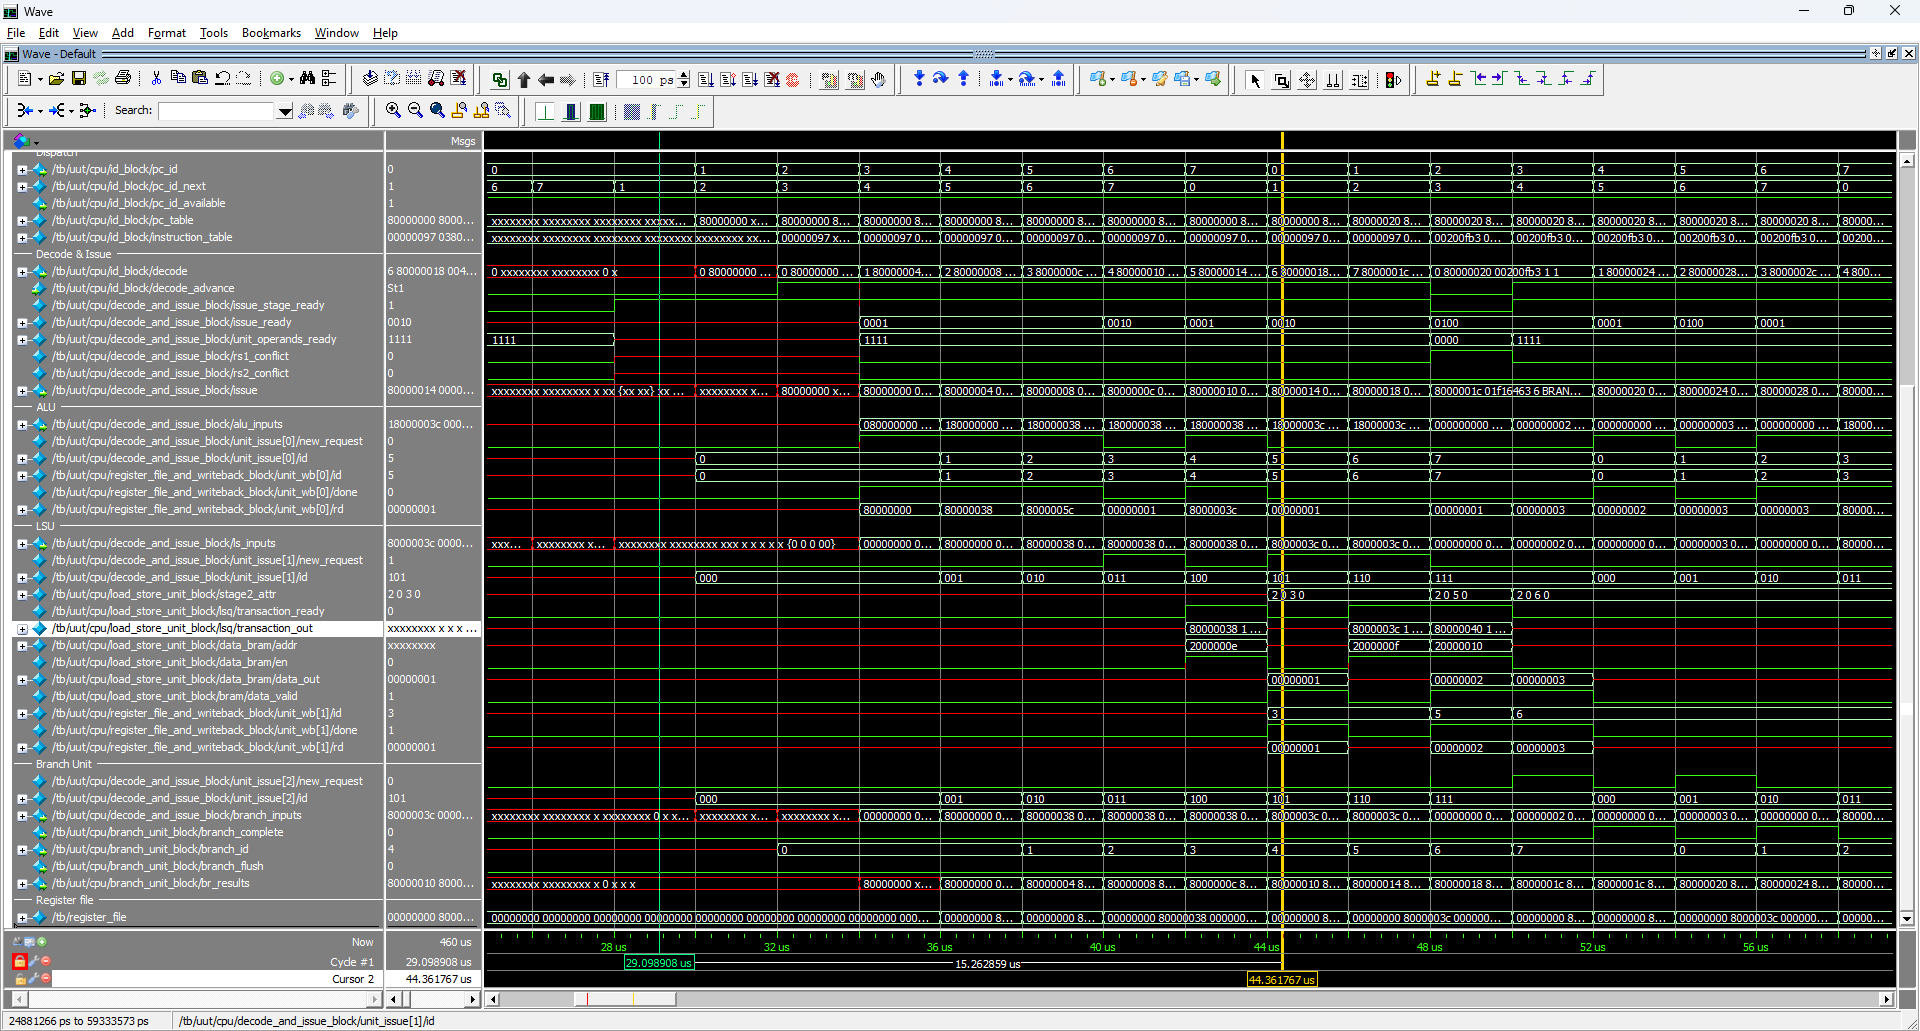
\includegraphics[scale=0.25]{images/05-decode.png}
 \captionof{figure}{Временная диаграмма сигналов команды lw x3, 4(x1) на стадии декодирования}
\end{center}

\begin{center}
\centering 
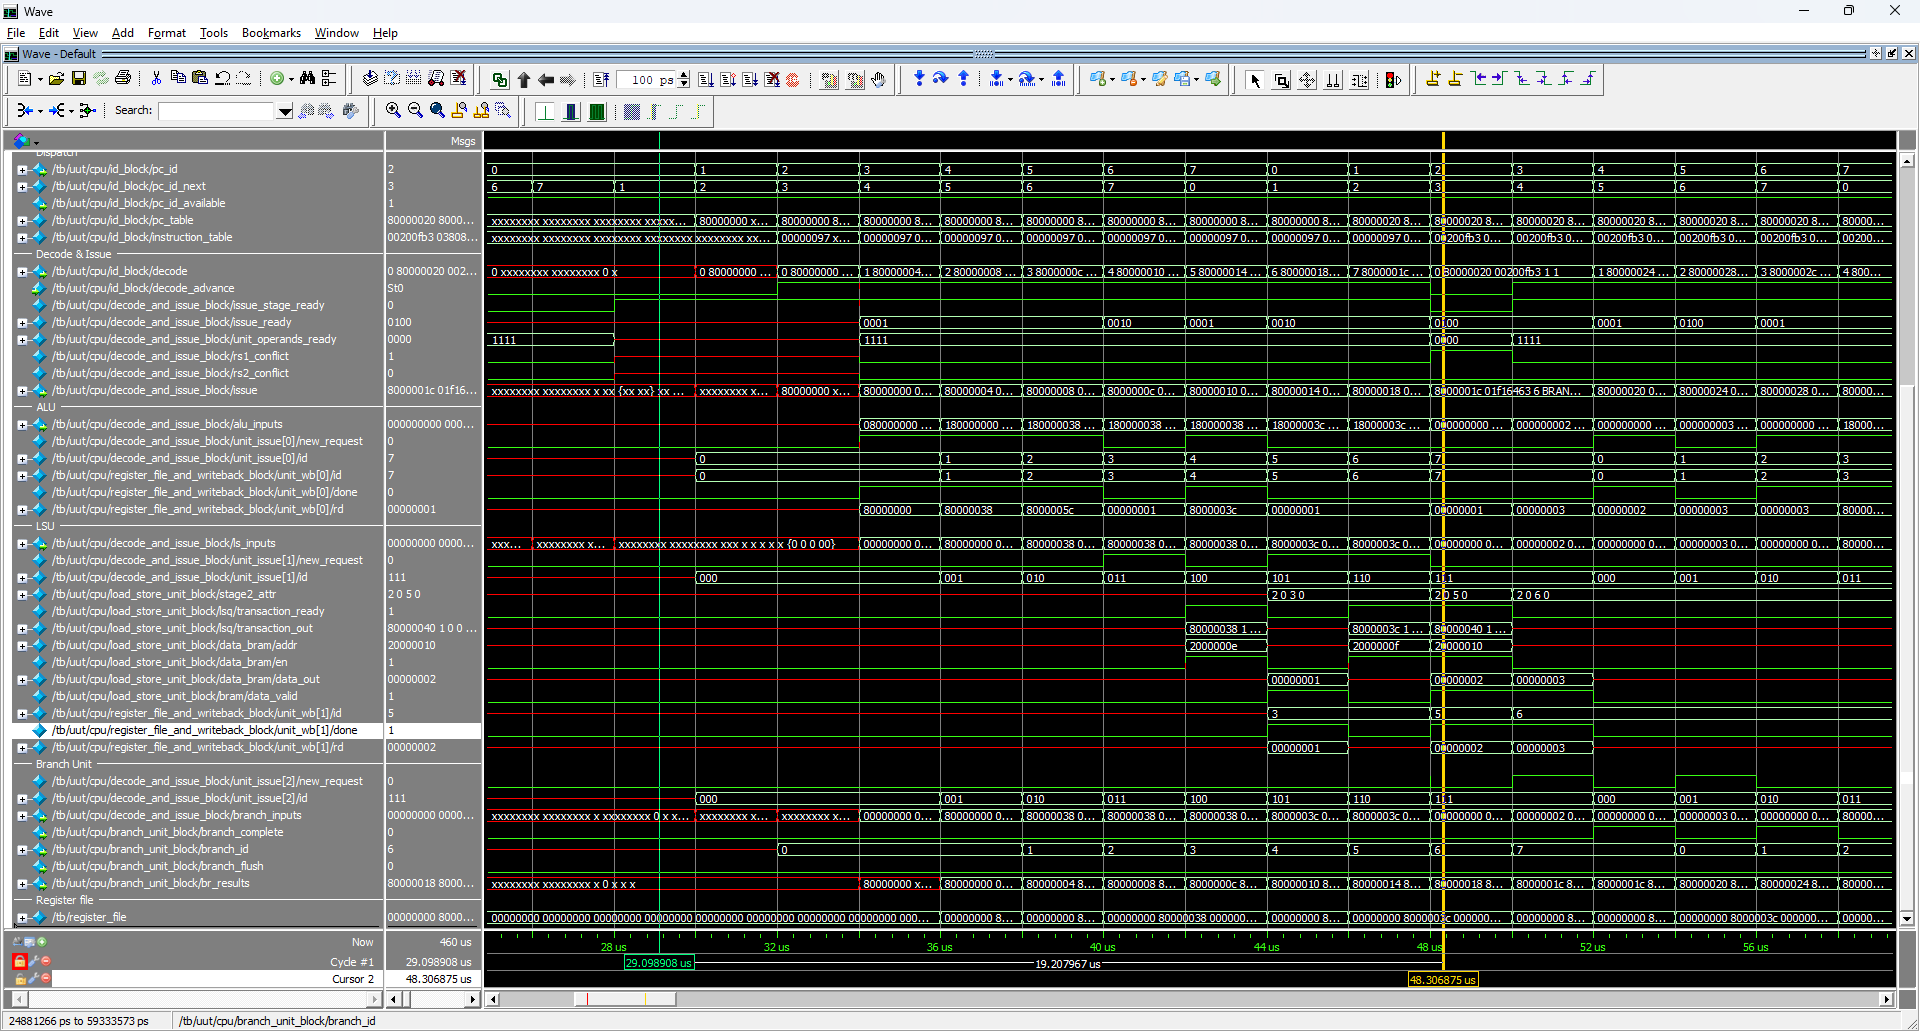
\includegraphics[scale=0.25]{images/05-execute.png}
 \captionof{figure}{Временная диаграмма сигналов команды lw x3, 4(x1) на стадии выполнения}
\end{center}

Программа достаточно хорошо оптимизирована, так как планирование производилось более чем на 75\% тактах. Если же попробовать, к примеру, поменять в цикле порядок загрузки значения в регистр и ветвления, то эффективность программы снизится.

\begin{center}
\centering 
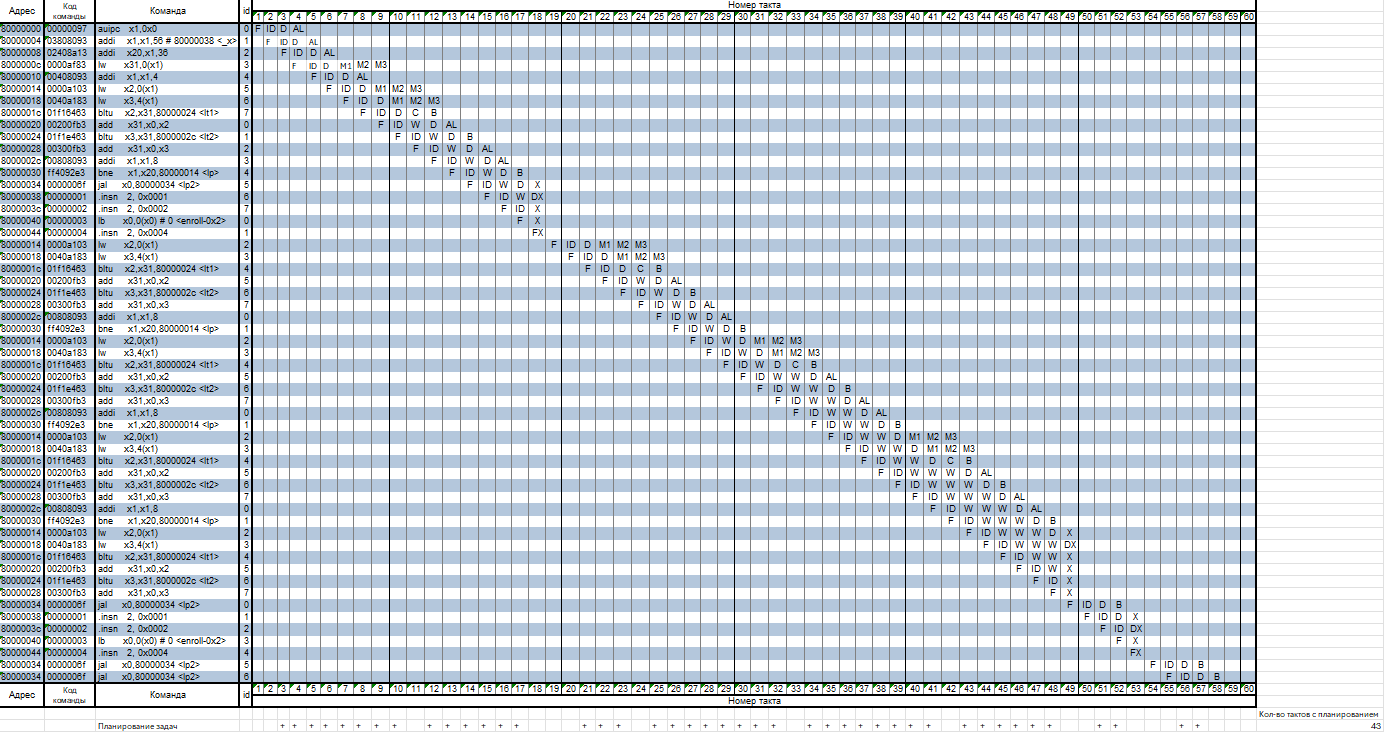
\includegraphics[scale=0.35]{images/05-route.png}
 \captionof{figure}{Трасса работы программы}
\end{center}